\documentclass[table,CJK,mathserif,notheorem,10pt]{beamer}% notheorems,

\usepackage{units}
\usepackage{float}
\providecommand{\tabularnewline}{\\}
\usepackage{colortbl}
\usepackage{graphicx} 
\usepackage{booktabs} % 导入三线表需要的宏包
\usepackage{multirow} 
\definecolor{mygray}{gray}{.8}
\definecolor{mycyan}{cmyk}{.3,0,0,0}
\usepackage{diagbox}


%\usepackage[width=2cm,dark,tab]{beamerthemesidebar}
%\usepackage{colortbl} % ²ÊÉ«±í¸ñ
%\usepackage[table]{xcolor}
%\usepackage{booktabs} % ¿ÉÒÔʹÓÃÈýÏß±í
%\usepackage{multirow} % ¸´ÔÓ±í¸ñ£¬Ê¹ÓÃmultirow±ØÐë¼ÓÔظÃpackage
%\usepackage{dcolumn}
\usepackage{graphicx,subfigure,boxedminipage}
\usepackage{bm}
\usepackage{amsmath}
\usepackage[english]{babel}
% or whatever
\usepackage{CJK}
\usepackage[latin1]{inputenc}
% or whatever
\usepackage{alltt}
\usepackage{amsmath,amssymb,amsfonts}
\usepackage{times}
\usepackage{multimedia}
\usepackage{color}% [usenames]
\usepackage{hyperref}
%\usepackage[T1]{fontenc}
\graphicspath {{figure/}}%ͼƬËùÔÚµÄĿ¼
\usepackage{multicol}    %ͬʱʹÓõ¥ÁкͶàÁУ¬ÈçÏÂ
\usepackage{multirow}
%%%\begin{multicols}{2}
%%%\end{multicols}
\usepackage{setspace} % µ÷Õû¼ä¾à
\usepackage{boiboites} % ×Ô¶¨Ò嶨Àí»·¾³
\usepackage{textpos} % ʹlogo²»±»¸²¸Ç
%\begin{spacing}{1.5}
%\tableofcontents \listoffigures \listoftables
%\end{spacing}

\setlength{\columnsep}{-0.05cm} %Ë«À¸Ö®¼äµÄ¼ä¾à
%\setlength{\parskip}{-0.1\baselineskip} % ÉèÖöμä¾à

%%%%%%%%%%%%%%%%%%%%%%%%%%%%%%%%%%%%%%%%%%% Ä£°åģʽ¶¨Òå %%%%%%%%%%%%%%%%%%%%%%%%%%%%%%%%%%%%%%%%%%%
\mode<presentation> {
  \usetheme{CambridgeUS}   %[hideothersubsections] beamer Ä£°åµÄģʽ
  % Warsaw or ...,Antibes,PaloAlto,Darmstadt,Frankfurt,Boadilla,Antibes,Luebeck,CambridgeUS,Rochester

%%  With navigation bar: default, boxes, Bergen, Madrid, Pittsburgh, Rochester
%%  With a treelike navigation bar: Antibes, JuanLesPins, Montpellier.
%%  With a TOC sidebar: Berkeley, PaloAlto, Goettingen, Marburg, Hannover
%%  With a mini frame navigation: Berlin, Ilmenau, Dresden, Darmstadt, Frankfurt, Singapore, Szeged
%%  With section and subsection titles: Copenhagen, Luebeck, Malmoe, Warsaw

%% Latex ÉèÖÃ×ÖÌå´óСÃüÁîÓÉСµ½´óÒÀ´ÎΪ£º\tiny \scriptsize \footnotesize \small \normalsize \large \Large \LARGE \huge \Huge
%\definecolor{logo_color}{rgb}{191,22,94}

%  \usefonttheme[onlylarge]{structuresmallcapsserif}%
%  \usefonttheme[onlysmall]{structurebold}%
%  \usefonttheme{serif} % Times New Rome ×ÖÌå
  \usecolortheme{dolphin} % default¶¨Òå×óÉÏÌõ¿ò
  \usecolortheme[RGB={191,22,94}]{structure}
%% Inner color themes, ÆäËûÑ¡Ôñ: orchid,albatross,beaver,beetle,default,crane,dolphin,dove,fly,orchid,lily,rose,seagull,seahorse
%% Inner color themes, ÆäËûÑ¡Ôñ: sidebartab,whale,wolverine

  \useinnertheme{rectangles} % default,circles,margin,rounded,rectangles
%%  \useoutertheme{split} % default£¬infolines£¬miniframes,shadow,smoothbars,smoothtree,tree,sidebar

%  \useoutertheme[height=0.1\textwidth,width=0.15\textwidth,hideothersubsections]{sidebar}
  \setbeamercovered{transparent} % dynamic,transparent,invisible
  % or whatever (possibly just delete it)
}

%%%%%%%%%%%%%%%%%%%%%%%%%%%%%%%%%%%%%%%%%%% ÑÕÉ«¶¨Òå %%%%%%%%%%%%%%%%%%%%%%%%%%%%%%%%%%%%%%%%%%%
%% beamerÖÐÒѾ­¶¨ÒåµÄÑÕÉ«£º
%% red,green,blue,cyan,magenty,yellow,black,darkgray,gray,lightgray,orange,violet,purple,brown

%% ×Ô¶¨ÒåÑÕÉ«£º
%% \xdefinecolor{lanvendar}{rgb}{0.8,0.6,1}
%% \xdefinecolor{olive}{cmyk}{0.64,0,0.95,0.4}
 %\colorlet{structure}{blue!60!black}
% \colorlet{structure}{blue!85!white}      %  ×Ô¶¨ÒåÑÕÉ«,ÓÃ"structure"±íʾ 60%À¶É«+40%ºÚÉ«µÄÑÕÉ«

%\setbeamertemplate{background canvas}[vertical shading][bottom=white,top=structure.fg!25] %%±³¾°É«, ÉÏ25%µÄÀ¶, ¹ý¶Éµ½Ï°×.
%\beamertemplateshadingbackground{white}{blue!25} %ÉèÖý¥±ä(gradient)±³¾°É«,
%\beamersetaveragebackground{yellow!25} % ÉèÖõ¥Ò»µÄ(solid)±³¾°É«
%\beamertemplategridbackground[0.3cm] % ÉèÖÃÕ¤¸ñ(grid ) ±³¾°

%%%%%%%%%%%%%%%%%%%%%%%%%%%%%%%%%%%%%%%%%%% ÏÔʾÉèÖà %%%%%%%%%%%%%%%%%%%%%%%%%%%%%%%%%%%%%%%%%%%
\def\hilite<#1>{\temporal<#1>{\color{white!80!black}}{\color{black}}{\color{white!50!black}}}% magenta
%% ×Ô¶¨ÒåÃüÁî, Ô´×Ô beamer_guide. item Öð²½ÏÔʾʱ, ʹ½«Òª³öÏÖµÄitem¡¢ÕýÔÚÏÔʾµÄitem¡¢ÒѾ­³öÏÖµÄitem¡¢ ³ÊÏÖ²»Í¬ÑÕÉ«.
% \hypersetup{pdfpagemode={FullScreen}} % ĬÈÏÈ«ÆÁ²¥·Å


% Or whatever. Note that the encoding and the font should match. If T1
% does not look nice, try deleting the line with the fontenc.

%%%%%%%%%%%%%%%%%%%%%%%%%%%%%%%%%%%%%%%%%%% Ò³ÃæÉèÖà %%%%%%%%%%%%%%%%%%%%%%%%%%%%%%%%%%%%%%%%%%%
\setbeamertemplate{navigation symbols}{}   %% È¥µôÒ³ÃæÏ·½Ä¬Èϵĵ¼º½Ìõ.
\setcounter{tocdepth}{2} % Ö»Éú³É2¼¶Ä¿Â¼
\setcounter{secnumdepth}{2}
\numberwithin{equation}{section} % ¹«Ê½°´Õ±àºÅ
%\numberwithin{equation}{subsection} % ¹«Ê½°´½Ú±àºÅ
\numberwithin{figure}{section} % ͼƬ°´Õ±àºÅ

\renewcommand{\raggedright}{\leftskip=0pt \rightskip=0pt plus 0cm} %  Á½¶Ë¶ÔÆë
\raggedright

\setbeamertemplate{caption}[numbered] % ͼ±í±àºÅ
\setbeamerfont{caption}{size=\footnotesize} %  ͼ±í±êÌâ×ÖÌå´óСÉèÖÃ

% µ÷ÕûµÚÒ»Ò³±êÌâռλ
% \defbeamertemplate*{frametitle}{smoothbars theme}
%  {
%    \nointerlineskip
%    \begin{beamercolorbox}[wd=\paperwidth,leftskip=.3cm,rightskip=.3cm plus1fil,vmode]{frametitle}
%      \vskip.6ex
%      \usebeamerfont*{frametitle}\insertframetitle%
%      \vskip.6ex
%    \end{beamercolorbox}
%  }

\pgfdeclaremask{cityu_logo}{figure/cityu_logo3}
\pgfdeclareimage[mask=cityu_logo,height=1cm,interpolate=true]{cityu_logo}{figure/cityu_logo3}
\addtobeamertemplate{frametitle}{}{%
%\begin{textblock*}{5cm}(.9\textwidth,-0.85cm)
\begin{textblock*}{5cm}(.88\textwidth,7cm) %%%µ÷½ÚlogoÔÚpptµÄλÖÃ
%
\includegraphics[height=1cm,width=1cm]{cityu_logo.pdf}
%bicong%\pgfuseimage{cityu_logo}
\end{textblock*}}

%%%%%%%%%%%%%%%%%%%%%%%%%%%%%%%%%%%%%%%%%%% ×Ô¶¨ÒåÒ³½Å %%%%%%%%%%%%%%%%%%%%%%%%%%%%%%%%%%%%%%%%%%%
\usefoottemplate{\hbox{\tinycolouredline{structure!80!black}{
\color{white}{ \insertshortauthor} \hfill{\insertshortinstitute }
\hfill{\footnotesize \insertframenumber\,/ \inserttotalframenumber}
% \hfill{{\the\year}/{\the\month}/{\the\day}}
}}}

%%%%%%%%%%%%%%%%%%%%%%%%%%%%%%%%%%%%%%%%%%% ÖÐÎÄ×ÖÌå %%%%%%%%%%%%%%%%%%%%%%%%%%%%%%%%%%%%%%%%%%%
\newcommand{\song}{\CJKfamily{song}}
\newcommand{\hei}{\CJKfamily{hei}}
\newcommand{\kai}{\CJKfamily{kai}}
\newcommand{\fs}{\CJKfamily{fs}}

%%%%%%%%%%%%%%%%%%%%%%%%%%%%%%%%%%%%%%%%%%% ÖÐÎĶ¨Àí»·¾³ %%%%%%%%%%%%%%%%%%%%%%%%%%%%%%%%%%%%%%%%%%%
%\newtheorem{theo}{{¶¨Àí}} % \begin{theo}  \end{theo}
%\newtheorem{prop}{{ÃüÌâ}}
%\newtheorem{lem}{{ÒýÀí}}
%\newtheorem{corol}{{ÍÆÂÛ}}[theorem]
%\newtheorem{def}{{¶¨Òå}}
%\newtheorem{exam}{{Àý}}

%%%%%%%%%%%%%%%%%%%%%%%%%%%%% ¶¨ÀíÃüÌâ±àºÅ %%%%%%%%%%%%%%%%%%%%%%%%%%%%%%%%%%
\setbeamertemplate{theorems}[numbered]
%\newtheorem{exam}{Example}[section] % °´Õ±àºÅ
\newboxedtheorem[background=lightgray]{exam}{Example}{section}

\newtheorem{coro}{Corollary}[section]
\newtheorem{thm}{Theorem}[section]
\newtheorem{lem}{Lemma}[section]
\newtheorem{exm}{Example}[section]
\newtheorem{rem}{Remark}[section]
\newtheorem{defi}{Definition}[section]
\newtheorem{prop}{Proposition}[section]

\newtheorem*{refer}{\vspace{-10pt}}
\newtheorem*{con}{Conclusion}
\newtheorem*{fw}{Future Work}
\newtheorem*{spo}{Sponsors}

\newcommand{\EQ}{\begin{eqnarray}}
\newcommand{\EN}{\end{eqnarray}}
\newcommand{\EQQ}{\begin{eqnarray*}}
\newcommand{\ENN}{\end{eqnarray*}}
\newcommand{\BM}{\left[\begin{array}}
\newcommand{\EM}{\end{array}\right]}
\newcommand{\upcite}[1]{$^{\mbox{\scriptsize \cite{#1}}}$}



\newcommand{\nnum}{\nonumber}
\newcommand{\ebox}{\hfill \rule{1.5mm}{1.5mm}}

\def \T{{\mbox{\tiny T}}}
\def \R{{\mbox{\tiny R}}}
\def \RR{{\mathbb{R}}}

\newcommand{\bdefinition}{\begin{defi} \begin{rm} }
\newcommand{\edefinition}{ \end{rm}
\end{defi} }
\newcommand{\bremark}{\begin{rem} \begin{rm} }
\newcommand{\eremark}{ \end{rm}
\end{rem} }
\newcommand{\btheorem}{\begin{thm}  \begin{rm} }
\newcommand{\etheorem}{ \end{rm}
\end{thm} }
\newcommand{\blemma}{\begin{lem} \begin{rm} }
\newcommand{\elemma}{ \end{rm}
\end{lem} }
\newcommand{\bcorollary}{\begin{coro} \begin{rm} }
\newcommand{\ecorollary}{ \end{rm}
\end{coro} }
\newcommand{\bproposition}{\begin{prop} \begin{rm} }
\newcommand{\eproposition}{ \end{rm}
\end{prop} }

\newcommand{\breference}{\begin{refer} \begin{rm} }
\newcommand{\ereference}{ \end{rm}
\end{refer} }

\newcommand{\bconclusion}{\begin{con} \begin{rm} }
\newcommand{\econclusion}{ \end{rm}
\end{con} }

\newcommand{\bfw}{\begin{fw} \begin{rm} }
\newcommand{\efw}{ \end{rm}
\end{fw} }

\newcommand{\bspo}{\begin{spo} \begin{rm} }
\newcommand{\espo}{ \end{rm}
\end{spo} } 


\large
\title[My Title]{Overview on Noncooperative Games and Distributed Nash Equilibrium Seeking over Multi-Agent Networks}

\author[]{PhD Student: Binghao OuYang \\ \vspace{1em} Supervisor: Prof. FENG, Gang, Prof. WANG, Yong}

\institute[Department of Biomedical Engineering, City University of Hong Kong]{Department of Biomedical Engineering\\ City University of Hong Kong}

\date{\scriptsize{February 10, 2023}}

\begin{document}

\begin{CJK}{GBK}{kai}

\begin{frame}
\begin{figure}
\begin{center}

\includegraphics[height=2cm]{figure/cityu_logo2}
\end{center}                                 
\end{figure}
  \titlepage

\end{frame}

\AtBeginSection[] {
  \begin{frame}<beamer>
    \frametitle{Outline}
    \tableofcontents[currentsection]
  \end{frame}
}

\begin{frame}{Outline}
  \tableofcontents
\end{frame}

%%%%%%%%%%%%%%%%%%%%%%%%%%%%%%%%%%%%%%%%%%%%%%%%%%%%%%%%%%%%%%%%%
\section{Introduction}\label{sec:1}

\subsection[Research background]{Research background}\label{subsec:1-1}
\begin{frame}
\frametitle{\normalsize{Background}}\transwipe
      % \breference
      % [1] E. Fridman, ``Introduction to Time-Delay Systems: Analysis and Control,''  \emph{Springer,} pp.~22-28, 2014.
      % \ereference
 \begin{itemize}
  \item With the rapid development of wireless communication technology, various kinds of large-scale network systems are increasingly applied in the fields of engineering technology. Thus, comes the problem of how to make interconnected multi-agent work together.
  \vspace{0.4cm}
  \begin{columns}[c]
 \column{6cm}
   \begin{figure}
       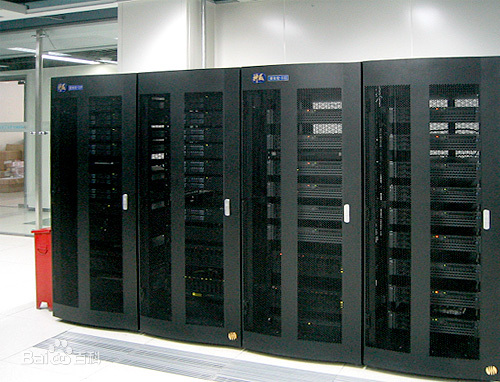
\includegraphics[height=0.7in]{figure/game/1-computer_cluster.jpg}
       \vspace{-6pt}
       \caption{computer clusters}
      \label{fig1}
   \end{figure}
    \column{6cm}
    \begin{figure}
      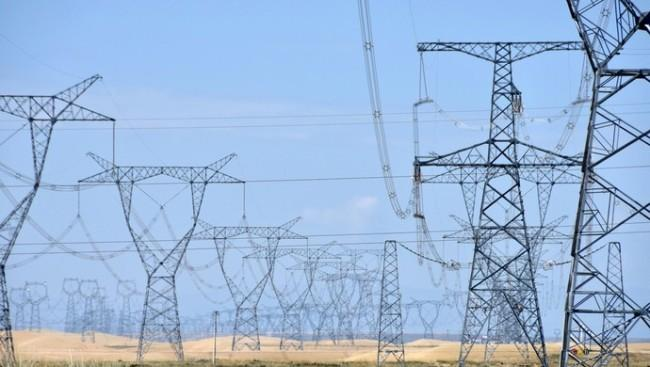
\includegraphics[height=0.7in]{figure/game/2-multi-microgrid.jpeg}
      \vspace{-6pt}
      \caption{multi-microgrid systems}
     \label{fig2} 
  \end{figure}
    \end{columns}

  \begin{columns}[c]
    \column{6cm}
      \begin{figure}
          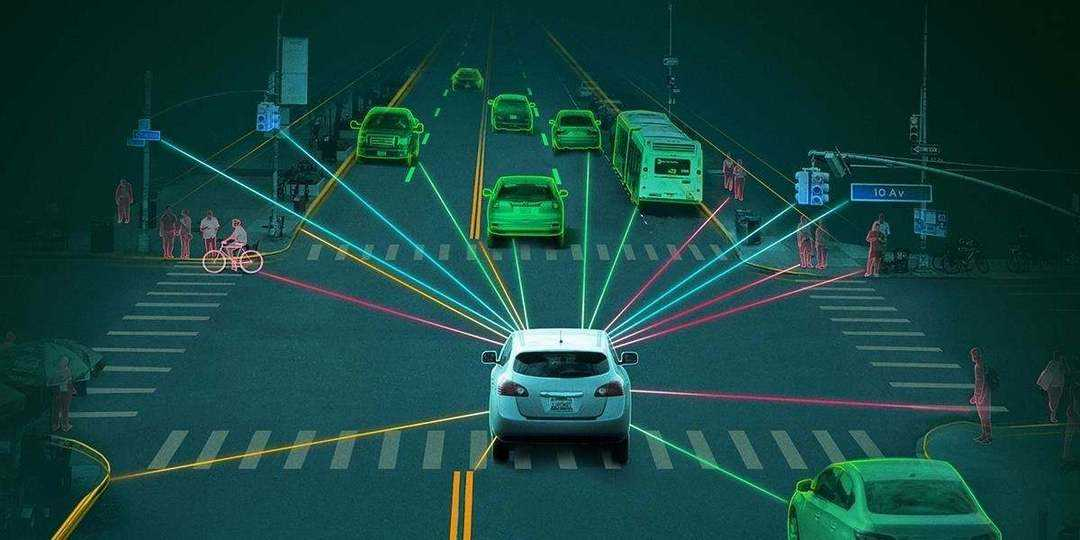
\includegraphics[height=0.7in]{figure/game/3-autonomus-driving.jpeg}
          \vspace{-6pt}
          \caption{autonomous driving networks}
         \label{fig3}
      \end{figure}
       \column{6cm}
       \begin{figure}
         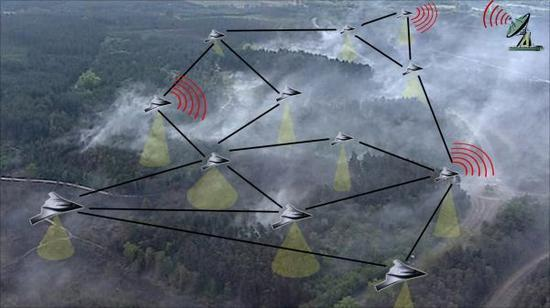
\includegraphics[height=0.7in]{figure/game/4-UAV-systems.jpeg}
         \vspace{-6pt}
         \caption{UAV systems}
        \label{fig4} 
     \end{figure}
       \end{columns}

  \end{itemize}
\end{frame}

\subsection[Game Theory]{Game theory in multi-agent}\label{subsec:1-2}

\begin{frame}
\frametitle{\normalsize{Game theory in multi-agent}}\transwipe

\begin{itemize}
\item \textcolor[rgb]{0.00,0.00,1.00}{Game theory}, which studies the cooperation and conflict among multiple rational decision makers, called players, can be utilized to analyze a large class of engineering system.
\item In general multi-agent problems, the global cost function as follows. $f_i(x)$ is the local cost function depends on $x_i$, we try to minimize global cost function.
\vspace{6pt}
\begin{equation}
\begin{split}
 J(x)=\sum_{i=1}^N f_i(x), x=\left[x^1, \ldots, x^m\right]^T \in \mathbb{R}^m
\end{split}
\end{equation}

\item In game theroy problems, the players’ objective functions are dependent on \textcolor[rgb]{0.00,0.00,1.00}{other players’ actions}, which lead to the coupling between the players’ actions in the decision-making process. 
 \vspace{6pt}
 \begin{equation}
 \begin{split}
  \min _{x_i \in \mathbb{R}_i} J_i\left(x_i, x_{-i}\right), \quad \text { s.t. } \quad x_i \in X_i \end{split}
 \end{equation}
\end{itemize}
\breference
\scriptsize
[1]Z. M. Fadlullah, "A survey of game theoretic approaches in smart grid," WCSP, 2011, pp. 1-4.\par
\ereference
\end{frame}


\begin{frame}
\frametitle{\normalsize{Nash Equilibrium}}\transwipe
\begin{itemize}

\item An action $x^\star$ is defined as an \textcolor[rgb]{0.00,0.00,1.00}{Nash Equilibrium} of the game G(N, $J_i$), if for all i $\in N$
\begin{equation}
  J_i\left(x_i^*, x_{-i}^*\right) \leq J_i\left(x_i, x_{-i}^*\right)
\end{equation}
Let $x_i$ be player i's action and $x_{-i}$ represent other players’ actions.
\vspace{6pt}

\item From the above definition, none of the agents can benefit from \textcolor[rgb]{0.00,0.00,1.00}{unilaterally} changing its strategy at NE conditions.
\vspace{6pt}

\item Because if one player changes it's strategy, others will also change their strategies, which leads to a increasement of cost function. 

% \item In order to reach NE, every agent needs to consider the actions of other agents.


\end{itemize}

% Let $\beta \geq r \geq 0$ be given real numbers($\beta$ may be $+\infty$), $E^n$ be an n-dimensional linear vector space with a seminorm $|\cdot|$, $p:[-\beta,0]\to (0, \infty)$ be Lebesque integrable on $[-\beta,0]$, positive and nondecreasing on $[-\beta,0]$.Let $\mathcal{B}=\mathcal{B}([-\beta,0], E^n)$ be the Banach sapce of functions which are continuous on $[-r,0]$ and such that 
% \begin{equation}
% |\phi|=\sup_{\theta \in [-r,0]}|\phi(\theta)|+\int^0_{-\beta}p(\theta)|\phi(\theta)|d\theta <\infty
% \end{equation}
\end{frame}

\section[Distributed Nash equilibrium seeking over networks]{Distributed Nash equilibrium seeking over networks}\label{sec:2}

\subsection[Mathematical models of different game structure]{Mathematical models of different game structure}\label{subsec:2-2}

\begin{frame}
  \frametitle{\normalsize{Monotone game}}
  \begin{itemize}\small


      \item A game is called monotone game if it satisfies the following condition: \\
      $$ F(x) \triangleq (\bigtriangledown _{x_1}^T J_1 (x_1),\cdots , \bigtriangledown _{x_N}^T J_N (x_N) ) $$
      $$(F(x)-F(y))(x-y) \geqslant 0$$
      Where $J_i$ represents player i's cost function, F(x) denote the pseudo-gradient of the game.
      \vspace*{6pt} \\
      \item In monotone game, the NE is \textcolor[rgb]{0.00,0.00,1.00}{ unique and always exists.}
      \vspace*{6pt} \\
      \item Most of current work requires the game is monotone, and it's a basical assumption.
  \end{itemize} 
        
\end{frame}


\begin{frame}
  \frametitle{\normalsize{Generalized Nash game}}
  \begin{itemize}\small


      \item In many practical engineering networks, the player strategies are usually required to satisfy certain \textcolor[rgb]{0.00,0.00,1.00}{coupling constrain}. Generalized Nash game is used to solve these problems.
      \item  Compared with the Nash equilibrium problem mentioned before, there are constraints between agents' actions.
      \begin{equation}
        \min _{x_i \in \mathbb{R}} J_i(x) \text {, such that } g(x) \leq 0 \text {}
      \end{equation}
      where g(x) is constraint function.
      
      \item There are four type of constraints in generalized Nash game.
      
      \begin{itemize}
        \item Type I (Set Constraint) : Each player’s action is limited within a required and predefined domain. ie $x_i \in [x^{min}_i, x^{max}_i]$
        \item Type II (Linear Equality Constraint) : $$c^{T} \mathbf{x}-d=0 \text { or } \sum_{i=1}^{N} A_{i} x_{i}=\sum_{i=1}^{N} b_{i}$$
        \item Type III/IV (Nonlinear Inequality) : Type III constraint only involves
        each player’s local action, while Type IV is a class of nonlinear constraint that
        may involve all players’ actions
      \end{itemize}
      
  \end{itemize} 
        
\end{frame}

\begin{frame}
  \frametitle{\normalsize{Aggregative Games}}\small

\begin{itemize}
  \item 
  In an aggregative game, the cost function of the player is
  composed of local functions that depend on the player itself
  and \textcolor[rgb]{0.00,0.00,1.00}{the sum of other players' local functions}.
  \begin{columns}[c]
    \column{6cm}
      \begin{figure}
          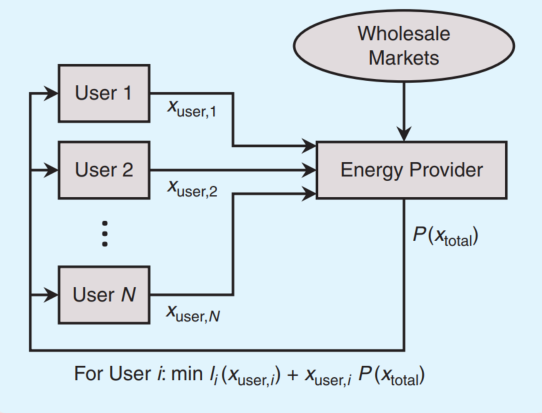
\includegraphics[height=1.5in]{figure/game/2-aggregative.png}
          \vspace{-6pt}
          \caption{ Aggregative Game}
      \end{figure}
      \column{6cm}
      \begin{equation}
        \begin{aligned}
        J_i = I_i(X_{user, i}) + X_{user, i} P(X_{total})
        \end{aligned}
        \end{equation}
    The objective of each electricity user is to minimize $J_i$which depends on its own energy consumption $X_{user,i}$ and the sum of all users’ energy consumption $X_{total}$.
  
    \item The aggregative game problems don't need to estimate all agents’ strategies, but require each agent to estimate the \textcolor[rgb]{0.00,0.00,1.00}{aggregation function} P.

    \end{columns}
\end{itemize}
\end{frame}


\begin{frame}
  \frametitle{\normalsize{Other Game Models}}\small
\begin{itemize}
  \item \textcolor[rgb]{1.00,0.00,0.00}{Other game models}
  
  There are also other distribute game models widely studied.
\end{itemize}

\begin{tabular}{cp{8cm}}% 其中,tabular是表格内容的环境;c表示centering,即文本格式居中;c的个数代表列的个数
	% \renewcommand\arraystretch{2}
  \toprule %[2pt]设置线宽     
  \centering
  Game models & Description \\
  \midrule %[2pt]  
 Zero-sum Games & The income of one player will inevitably lead to the loss of the other player. \\  \hline
  Potential Games & The change of single agent's local function and global function are equal.  $P\left(x_{i}, x_{-i}\right)-P\left(x_{i}^{\prime}, x_{-i}\right)=J_{i}\left(x_{i}, x_{-i}\right)-J_{i}\left(x_{i}^{\prime}, x_{-i}\right), \quad \forall x_{i}, x_{i}^{\prime} \in X_{i}$  \\
  \hline  Online Games & It refers to the adaptive decision making in repeated
  games. \\ \hline
  N-Coalition Games & Each coalition consisting of multiple agents collectively acts  as a virtual player to minimize the coalition cost function. \\
  \hline Gradient-Free Games &  The relation between the action variables and the cost functions is unknown. \\
  \bottomrule %[2pt]     
  \end{tabular}

  \breference
  \scriptsize
  [2]P. Yi, "A Survey on Noncooperative Games and Distributed Nash Equilibrium Seeking over Multi-Agent Networks
  " CAAI Artificial Intelligence Research 2022 Vol. 1 Issue 1 Pages 8-27
  \ereference
\end{frame}






\subsection[Nash equilibrium seeking algorithms]{Nash equilibrium seeking algorithms}\label{subsec:2-3}
\begin{frame}
  \frametitle{\normalsize\textsc{Consensus problem}}\transwipe
  
  \begin{itemize}
    \item In centrallized system, every agent know others' actions, so it's easy to calculates NE.
    \item In distributed systems, agents can only have an access to \textcolor[rgb]{0.00,0.00,1.00}{partial decision information}
    from its neighborhood agents, so they need communicate and exchange information through connected network to reach consensus.
    \item The \textcolor[rgb]{0.00,0.00,1.00}{leader-following} consensus technique has been widely used to reach consensus in distributed NE seeking
    \item The core idea of the strategy is that each player makes a local estimate of the unknown players’ actions by utilizing a leaderfollowing consensus protocol. 
    \begin{equation}
    \dot{y}_{i j}=-k_{i j}\left(\sum_{k=1}^{N} a_{i k}\left(y_{i j}-y_{k j}\right)+a_{i j}\left(y_{i j}-x_{j}\right)\right)
     \end{equation}

    where $y_{ij}$ represents agent i's estimation on agent j's action.
    \end{itemize}
  \end{frame}
  
\begin{frame}
  \frametitle{\normalsize\textsc{Nash equilibrium Seeking}}\transwipe
  
  \begin{itemize}
    \item Once consensus reached, it's easy to find NE just like centrallized systems.
    \item The gradient-like algorithm is adopted to update the players’ actions to reach NE.
     \begin{equation}
      \dot{x}_i  =-k_i \nabla_{x_i} J_i\left(y_i\right)
    \end{equation}
     It can replacing x in the gradients with $y_i$ for each agent, because agents update their actions based on their estimations.
    
     \item In fact,  agents' updation based on a combination of consensus and NE seeking module. To ensure the stability of the closed-loop system, a small positive parameter is included in the gradient part to ensure that the consensus part is faster than the gradient optimization part, thus forming a \textcolor[rgb]{0.00,0.00,1.00}{two time-scale structure}.
     
     \item The speed of consensus part is closely related to the communication network.
  \end{itemize}

  \end{frame}


\begin{frame}
    \frametitle{\normalsize\textsc{Graph Structure}}\transwipe
    
    \begin{itemize}
      \item When the communication graph is connected, the quasisteady state of the leader-following consensus part is $y_i = x$. But the \textcolor[rgb]{0.00,0.00,1.00}{convergence speed} is highly depends on graph's connectivity. The eigenvalue of graph's Laplacian matrix can used to convergence analysis.
      \item \textcolor[rgb]{1.00,0.00,0.00}{ Undirected Graph}\\
       Let $\lambda_{n}$ represent the eigenvalues of Laplacian matrix $\mathcal{L}$. When graph is connected, we have \\
      \begin{columns}[c]
        \column{6cm}
          \begin{figure}
              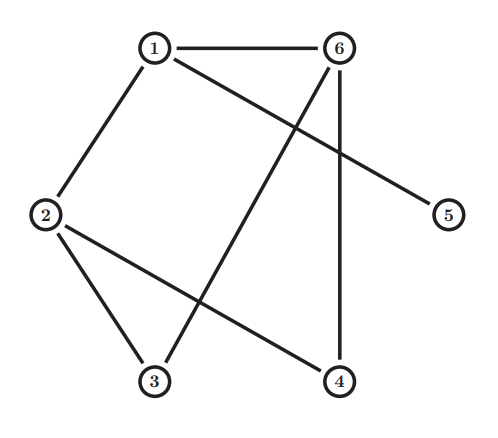
\includegraphics[height=1.2in]{figure/game/2-undirecti.png}
              \vspace{-6pt}
              \caption{ Undirected graph}
          \end{figure}
          \column{6cm}
          \begin{equation}
            \begin{aligned}
              \mathcal{L} &:=D-\mathcal{A} \\ 
              \lambda_{2} & > 0 \\
              \lambda_{1} & = 0 \\
              \lambda_{n} & \geq d_{\max }+1 \\ 
              0 \leq \lambda_{1} \leq \lambda_{2} &\leq \ldots \leq \lambda_{n}.\\ 
            \end{aligned}
            \end{equation}
         Where D is degree matrix, A is adjacency matrix. $\mathcal{L}$ is symmetric semi-positive definite, $d_{max}$ represents the maximum degrees in graph. 
        \end{columns}

    \end{itemize}
  
\end{frame}

\begin{frame}
  \frametitle{\normalsize\textsc{Graph Structure}}\transwipe
      \begin{itemize}
      \item \textcolor[rgb]{1.00,0.00,0.00}{ Directed Graph}\\
      \begin{columns}[c]
        \column{6cm}
          \begin{figure}
              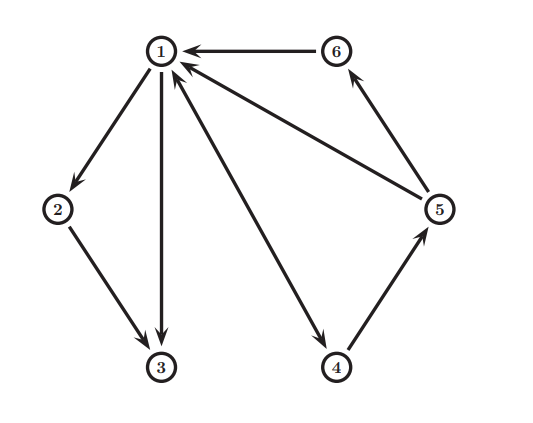
\includegraphics[height=1.2in]{figure/game/2-directi.png}
              \vspace{-6pt}
              \caption{ Directed graph}
          \end{figure}
          \column{6cm}
          \begin{equation}
            \begin{aligned}
              &\mathcal{L} :=D_{in} -\mathcal{A} \\ 
              &R \mathcal{L}  +\mathcal{L}^{T} R \geq 0 \\
              &R =\operatorname{diag}\left(r_{1}, \cdots, r_{N}\right), r_i \ge 0\\
              &r^{T} \mathcal{L}=0 \text { and } r^{T} \mathbf{1}=1 \\ 
            \end{aligned}
            \end{equation}
        
        \item Where $D_{in}$ is in-degree matrix. r is left eigenvector of $\mathcal{L}$ associated with the zero eigenvalue.
        \item When graph is strong connected, r is unique. 
        \item The second equation widely used to convergence analysis, because $\mathcal{L}$ is indefinite matrix.
        \end{columns}
    \end{itemize}

\end{frame}



\begin{frame}
  \frametitle{\normalsize{Generalized Nash Equilibrium Seeking}}\small
  
\begin{itemize}

  \item For GNE seeking (in addition to estimating the actions), the multipliers of all players for the same constraint must be synchronized since finding a GNE where the Lagrangian multiplier of each player is different may be extremely hard.
  \begin{equation}
  \begin{aligned}
    \dot{x}_{i} & =-k_{i}\left(\nabla_{x_{i}} J_{i}\left(y_{i}\right)+\lambda_{i} \nabla_{x_{i}} g\left(y_{i}\right)\right) \\
    \dot{\lambda}_{1} & =k_{1} \lambda_{1} g\left(y_{1}\right)\\
    \dot{\lambda}_{i} & =-\gamma_{i} \sum_{k=1}^{N} a_{i k}\left(\lambda_{i}-\lambda_{k}\right), \\
    \dot{y}_{i j} & =-w_{i j} \sum_{k=1}^{N} a_{i k}\left(y_{i j}-y_{k j}\right), \quad j \in \mathcal{V} \backslash\{i\}
  \end{aligned}
  \end{equation}
  \item  player 1  calculates the common multiplier using second equation, and all of the
  other players estimate this multiplier using a leader-following consensus algorithm in third equation. In addition, last equation is
  for action estimation.
\end{itemize}
\end{frame}


\begin{frame}
  \frametitle{\normalsize{Nash Equilibrium Seeking in  Aggregative Games}}\small


\begin{itemize}
  \item To achieve distribute NE seeking, different from general Nash games, the aggregative game problem does not need to estimate all agents’ strategies, but only requires
  each agent to estimate the sum of players' local function.

  \begin{equation}
  \begin{aligned}
    \dot{x}_{i}&=\mathcal{P}_{\Omega_{i}}\left(x_{i}-G_{i}\left(x_{i}, \eta_{i}\right)-\frac{\gamma}{N} A_{i}^{\top} \lambda_{i}\right)-x_{i,} \\
    \dot{\lambda}_{i}&=\beta \sum_{j \in \mathcal{N}_{i}} \operatorname{sgn}\left(\lambda_{j}-\lambda_{i}\right)+\gamma\left(A_{i} x_{i}-b_{i}\right), \\
    \dot{\zeta}_{i}&=\alpha \sum_{j \in \mathcal{N}_{i}} \operatorname{sgn}\left(\eta_{j}-\eta_{i}\right), \\
    \eta_{i}&=\zeta_{i}+\phi_{i}\left(x_{i}\right),  
  \end{aligned}
  \end{equation}

  \item 
   $G_{i}\left(x_{i}, \eta_{i}\right):=\left.\nabla_{x_{i}} J_{i}(x)\right|_{\sigma(x)=\eta_{i}}, A=\left[A_{1}, \ldots, A_{N}\right], b=\sum_{i=1}^{N} b_{i} $.\\
  x represents the players' actions, $\lambda$ is the multiplier, $\zeta$ used to estimate others local cost function and $\eta$ is the sum of cost function.
\end{itemize}
\breference
\scriptsize
[3] G. Hu, ``Distributed Nash Equilibrium Seeking: Continuous-Time Control-Theoretic Approaches''  \emph{IEEE Control Systems Magazine }, 2022 Vol. 42 Issue 4 Pages 68-86.
\ereference
\end{frame}

\begin{frame}
\frametitle{\normalsize\textsc{Related Work}}\transwipe 
    
\begin{itemize}
    \item Here are related work about distributed Nash equilibrium seeking in different game structures and  we mainly focus on continuous-time.\\

      \begin{tabular}{ccccc}     \footnotesize
        \diagbox{Models}{Structure} & Constraint&  Undirected & Directed  & Varing \\
        \hline
        Generalized games & Type I/II/III/IV  & \checkmark & \checkmark &    \\
        \hline
        \multirow{2}{4em}{Aggregative games }&  Type I  &\checkmark & \checkmark& \\
        & Type II  &\checkmark &  &  \\ 

        \hline
        Zero-Sum games & NA &\checkmark & \checkmark &     \\
        \hline
        N-Coalition  games & NA  & \checkmark & \checkmark & \checkmark  \\

        \bottomrule %[2pt]     
      
    \end{tabular}

    \end{itemize}
    \breference
    \scriptsize
    [4]Z. Li and Z. Duan, Cooperative Control of Multi-Agent Systems:
    A Consensus Region Approach. Boca Raton, FL, USA: CRC Press, 2017  \par
    [5]M. Ye, Q.-L. Han, L. Ding and S. Xu, Distributed Nash Equilibrium Seeking in Games With Partial Decision Information: A Survey, IEEE 2023 Pages 1-18
    \ereference
  \end{frame}

%%%%%%%%%%%%%%%%%%%%%%%%%%%%%%%%%%%%%%%%%%%%%%%%%%%%%%%%%%%%%%%%%
\section[Distributed settle time related Nash Equilibrium Seeking]{Distributed settle time related Nash Equilibrium Seeking}\label{sec:4}

\subsection[Prescribed-Time Control]{Prescribed-Time Control}\label{subsec:4-1}
\begin{frame}
\frametitle{\normalsize{Prescribed-Time Control}}\transwipe
According to the settle time of the control system, we can divide the control types into the following types.
\begin{itemize}
    \item Finite-time control: the settling time is related to \textcolor[rgb]{0.00, 0.00, 1.00}{initial conditions}  and design parameters
     \vspace{6pt}
    \item Fixed-time control: the settling time can be estimated by an \textcolor[rgb]{0.00, 0.00, 1.00}{upper bounded} function independent of initial conditions.
    \vspace{6pt}
    \item Predefined-time control: the upper bound of the settling time can be \textcolor[rgb]{0.00, 0.00, 1.00}{user-set} freely.
    \vspace{6pt}
    \item Prescribed-time control: the exact settling time can be \textcolor[rgb]{0.00, 0.00, 1.00}{user-assigned arbitrarily}.
\end{itemize}
\end{frame}


\begin{frame}
\frametitle{\normalsize{Prescribed-Time Control}}\transwipe
\begin{figure}
  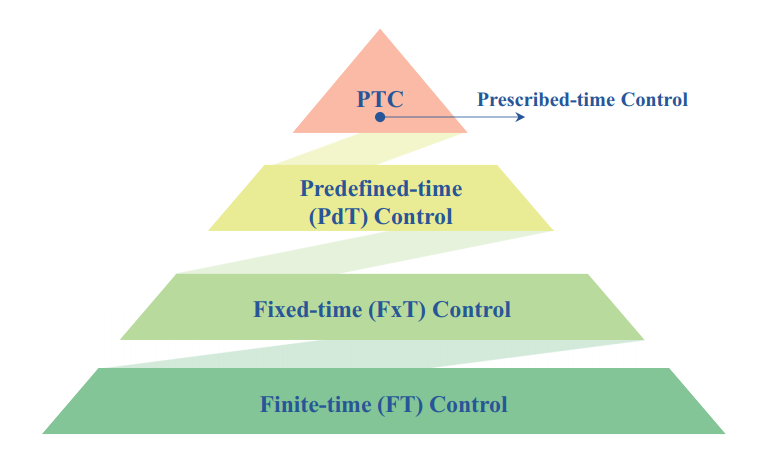
\includegraphics[height=1.5in]{figure/game/3-ptc.png}
  \vspace{6pt}
  \caption{The relationships among FT/FxT/PdT and PT control}
\end{figure}
\bremark
The most ideal and difficult one is PT control.
\eremark
\end{frame}

\begin{frame}
  \frametitle{\normalsize{Prescribed-Time Control Design}}\transwipe
  \begin{figure}
    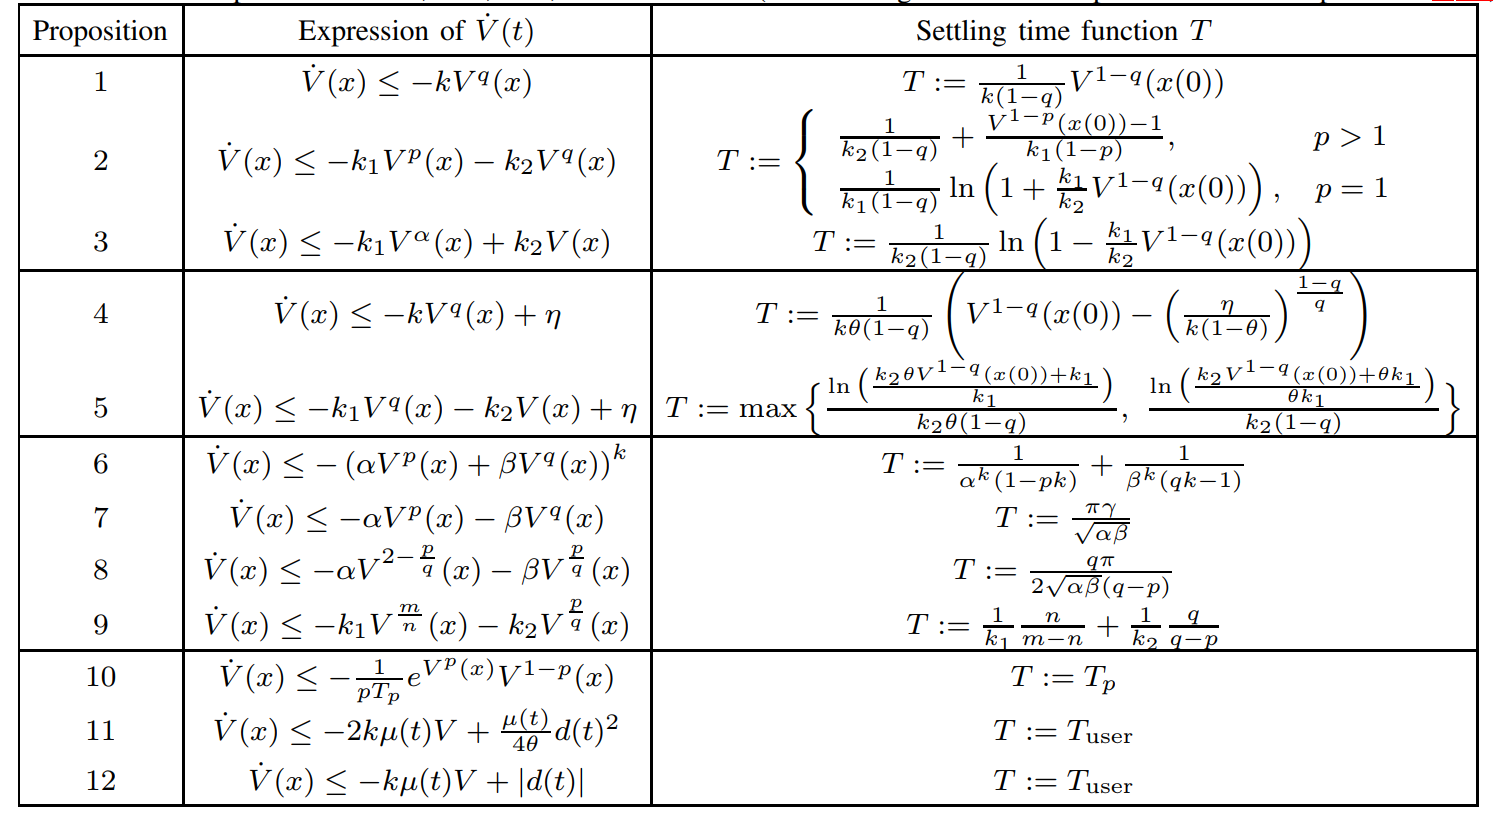
\includegraphics[height=1.85in]{figure/game/3-ptcd.png}
    \vspace{6pt}
    \caption{ Related Propositions on FT, FxT, PdT, and PT control}
  \end{figure}
  \bremark
  If the Lyapunov function satisfies the above conditions, we can get the corresponding settle  time control.
  \eremark
  \end{frame}
%%%%%%%%%%%%%%%%%%%%%%%%%%%%%%%%%%%%%%%%%%%%%%%%%%%%%%%%%%%%%%%%
\subsection[Fixed-Time Convergence for Distributed Nash Equilibrium Seeking]{Fixed-Time Convergence for Distributed Nash Equilibrium Seeking}
\begin{frame}
  \frametitle{\normalsize{Fixed-Time Convergence for Distributed Nash Equilibrium Seeking}}\transwipe
  
  \begin{itemize}\small
    \breference
    \scriptsize
    [5] Z. Li and Z. Ding, "Distributed Nash Equilibrium Searching via Fixed-Time Consensus-Based Algorithms," 2019 American Control Conference (ACC), 2019, pp. 2765-2770,
    \ereference
  \item This paper solves the  \textcolor[rgb]{0.00,0.00,1.00}{Fixed-Time} distributed Nash equilibrium searching problem with undirected graphs, which requires the graph to be \textcolor[rgb]{0.00,0.00,1.00}{strongly connected} and the cost function is \textcolor[rgb]{0.00,0.00,1.00}{m-strongly convex}.
  
  \item The control law for agent i is designed as 
  \begin{equation}
    \begin{aligned}
      \dot{\hat{x}}_{i i}= & \alpha \sum_{j=1}^{N} a_{i j} \operatorname{sig}\left(\hat{x}_{j i}-\hat{x}_{i i}\right)^{p}+\beta \sum_{j=1}^{N} a_{i j} \operatorname{sig}\left(\hat{x}_{j i}-\hat{x}_{i i}\right)^{q} \\
      & -\gamma\left[\operatorname{sig}\left(\nabla_{i} J_{i}\left(\hat{x}_{i}\right)\right)^{p}+\operatorname{sig}\left(\nabla_{i} J_{i}\left(\hat{x}_{i}\right)\right)^{q}\right] \\ 
      \dot{\hat{x}}_{i r}= &\alpha \sum_{j=1}^{N} a_{i j} \operatorname{sig}\left(\hat{x}_{j r}-\hat{x}_{i r}\right)^{p}+\beta \sum_{j=1}^{N} a_{i j} \operatorname{sig}\left(\hat{x}_{j r}-\hat{x}_{i r}\right)^{q}
    \end{aligned}
    \end{equation}
  Where  $\operatorname{sig}\left(x_{i}\right)^{p}=\operatorname{sign}\left(x_{i}\right)\left|x_{i}\right|^{p}$
  \end{itemize}

  \bremark
  $x_{ii}$ represents agent i's action, and for $r \neq i$, $x_{ir}$ represents agent i's state estimatation of agent j. 
  \eremark
  \end{frame}

  % Using above dynamic equation, agents can both reach consensus and reduce their cost functions.   

\begin{frame}
\frametitle{\normalsize{Convergence Analysis}}\transwipe

\begin{itemize}\small

\item The Lyapunov function set as follows
\begin{equation}
  \begin{aligned}
    V(t)= &\frac{1}{2} \sum_{i=1}^{N} \tilde{x}_{i}^{T} \tilde{x}_{i}\\
    \dot{V}_(t) \leq & -\left(\gamma m^{p} 2^{\frac{p+1}{2}}+\frac{1}{2} \alpha\left[4 \lambda_{2}\left(L_{B}\right)\right]^{\frac{p+1}{2}}\right) V_{3}^{\frac{p+1}{2}} \\
- & \left(\gamma m^{q} N^{\frac{-q^{2}-q+2}{2 q+2}} 2^{\frac{q+1}{2}}\right. \\
& \left.+\frac{1}{2} \beta N^{-\frac{-2 q^{2}-q+3}{2 q+2}}\left[4 \lambda_{2}\left(L_{C}\right)\right]^{\frac{q+1}{2}}\right) V_{3}^{\frac{q+1}{2}} .
  \end{aligned}
  \end{equation}
where $\tilde{x}_{i}=\hat{x}_{i}-x^{*}$, $x^{*}$  represents the Nash equilibrium point.

\item The Lyapunov function satisfies the fixed-time condition, and the settling time is obtained.
\end{itemize}
\bremark
$\lambda_{2} L_{C})$ represents the second
smallest eigenvalue of Laplacian matrix, which very important in both settling time and convergence analysis.
\eremark
\end{frame}
%%%%%%%%%%%%%%%%%%%%%%%%%%%%%%%%%%%%%%%%%%%%%%%%%%%%%%%%%%%%%

%%%%%%%%%%%%%%%%%%%%%%%%%%%%%%%%%%%%%%%%%%%%%%%%%%%%%%%%%%%%%
\begin{frame}
\frametitle{\normalsize{Current Work}}\transwipe
  \begin{itemize} \footnotesize

  \item There are only a few distributed Nash equilibrium search algorithms related to the convergence time.

  \begin{tabular}{cp{9cm}}
    \hline
    Papper & Description  \\
    \hline
    [6] & The papper design a non-cooperative distributed Nash equilibriums algorithm  in finite time \\ 
    \hline
    [7] & The papper proposed prescribed-time method for general directed graph. And each
    agent uses the information from the neighboring agents only at some sampling time instants.  \\  
    \hline
    [8] & The papper uses extremum seeking method to achieve semi-global practical fixed-time stability in model-free and time-varying graph scenario.\\
    \hline
    [9] & The papper proposed a adaptive NE seeking algorithm, where observer converges within FIXt while the NE seeking was asymptotically\\ 
    \hline
    [10] & The papper proposed prescribed convergence time algorithm over either fixed or switching communication topologies. \\
    \bottomrule %[2pt]     
    
\end{tabular}
  \end{itemize}
  \breference
  \scriptsize
  [6] X. Fang, Transactions on Applied Mathematics 2021 Vol. 2 Issue 1 Pages 162-174 \par
  % \ereference
  % \breference
  % \scriptsize
  [7] J. Zhou, Y. Lv and M. Ye 2021 60th IEEE Conference on Decision and Control (CDC) 2021\par
  % \ereference
  % \breference
  % \scriptsize
  [8] J. I. Poveda, M. Krstic and T. Basar IEEE Transactions on Automatic Control 2022 Pages 1-1.\par
  [9] Z. Li, Z. Li, and Z. Ding.  IEEE Transactions on Cybernetics, 2020 \par 
  [10] Z. Feng and G. Hu. 2020, arXiv preprint arXiv:2009.11649
  % [6] X. Fang, CSIAM Distributed Finite-Time Nash Equilibrium Seeking for Non-Cooperative Games   Transactions on Applied Mathematics 2021 Vol. 2 Issue 1 Pages 162-174 \par
  % % \ereference
  % % \breference
  % % \scriptsize
  % [7] J. Zhou, Y. Lv and M. Ye Appointed-time Distributed Nash Equilibrium Seeking for Networked Games 2021 60th IEEE Conference on Decision and Control (CDC) 2021\par
  % % \ereference
  % % \breference
  % % \scriptsize
  % [8] Fixed-Time Nash Equilibrium Seeking in Time-Varying Networks J. I. Poveda, M. Krstic and T. Basar IEEE Transactions on Automatic Control 2022 Pages 1-1.
  \ereference
\end{frame}
%%%%%%%%%%%%%%%%%%%%%%%%%%%%%%%%%%%%%%%%%%%%%%%%%%%%%%%%%%%%%%%%%
\section[Conclusions and future works]{Conclusions and future works}\label{sec:3}
%%%%%%%%%%%%%%%%%%%%%%%%%%%%%% ����Ŀ¼ҳ %%%%%%%%%%%%%%%%%%%%%%%%%%%%%%%%%%%
%\begin{frame}%<beamer>
%    \frametitle{\textsc{Contents}} \vspace{-1.05cm}
%    \begin{multicols}{2}
%    %\begin{figure}
%    \begin{minipage}[t]{0.4\textwidth}
%    \tableofcontents[currentsection,hideallsubsections]
%    % [currentsection,hideallsubsections][sectionstyle=show/shaded,subsectionstyle=show/shaded/hide]
%    \end{minipage}
%    \begin{minipage}[t]{0.6\textwidth}
%    \vspace{0.44cm}
%    \begin{spacing}{1.2} % ������� ��Ҫ\usepackage{setspace}
%%    \begin{itemize}
%%    \item\hyperlink{subsec:3-1}{Event-Triggered Control Scheme}
%%    \item\hyperlink{subsec:3-2}{Proof Idea}
%%    %\item\hyperlink{subsec:3-3}{Comparisons}
%%    \end{itemize}
%    \end{spacing}
%    \end{minipage}
%    %\end{figure}
%    \end{multicols}
%\end{frame}

%%%%%%%%%%%%%%%%%%%%%%%%%%%%%%%%%%%%%%%%%%%%%%%%%%%%%%%%%%%%%%%%%%
\begin{frame}
\frametitle{\normalsize{Conclusions}}\transwipe
    \begin{itemize}
        \vskip0.8em
        \item  Introduce game theroy problems.
        \vskip0.8em
        \item  Introduce Nash Equilibrium Seeking algorithms in different game models.
        \vskip0.8em
        \item  Introduce prescribed-time control problems and related distributed Nash Equilibrium Seeking algorithms.

    \end{itemize}
\end{frame}

%%%%%%%%%%%%%%%%%%%%%%%%%%%%%%%%%%%%%%%%%%%%%%%%%%%%%%%%%%%%%%%%%
\begin{frame}
\frametitle{\normalsize{Future works based prescribed-time NE seeking algorithms}}\transwipe
\begin{itemize}
    \item \textcolor[rgb]{1,0,0}{Information structure}
        \begin{itemize}
            \item  Solve fixed-time distributed Nash equilibrium Seeking problems with directed graph and time-varying graph. 
            \item  Propose fully distributed adaptive method without using global garph information. 
        \end{itemize} 
    \vspace{6pt}
    %\item The cooperative output regulation problems with infinite delays .
    \vspace{6pt}
    \item \textcolor[rgb]{1,0,0}{Game models} \\
    Extend prescribed-time control related algorithms to other game models like generalized Nash equilibrium games, aggregative games and so on.
    \vspace{6pt}
    
    \item \textcolor[rgb]{1,0,0}{Physical constraints} \\
    Combined with the actual physical model, consider the problems such as delay and disturbance in the process of distributed Nash equilibrium searching.
    %    \item Design some novel event-triggering mechanisms.
%    \vskip1em
%    \item Investigate adaptive distributed event-triggered control for MASs.
%    \vskip1em
\end{itemize}
\end{frame}
%%%%%%%%%%%%%%%%%%%%%%%%%%%%%%%%%%%%%%%%%%%%%%%%%%%%%%%%%%%%%%%%%



\section*{Acknowledgement\label{sec:9}}

\begin{frame}
\frametitle{\normalsize{Acknowledgement}}\transwipe
%\bspo
%\begin{itemize}
%\item \small UGC Block Grants and TA Scheme (UGC Funded)
%  \begin{figure}
%  \includegraphics[width=2.3in]{figure/ugc_logo}
%\end{figure}
%\end{itemize}
%\espo


\LARGE

\vspace{16pt}

~~~~~~~~~~~~~~~Thanks for your attention.


\end{frame} 


\end{CJK}
\end{document}
